\section{Tests de performances}

Pour tester les performances de notre programme, nous avons fait tourner le programme plusieurs fois, en partant d'une version full CPU, puis en augmentant peu à peu la part dédiée au GPU. Tous les tests ont été effectué sur une moyenne de temps de trois exécutions du programme.

	\subsection{Machines utilisées}

	Nous avons d'abord effectué les tests avec l'une de nos machines personnelles. Les résultats ne nous permettant pas de tirer des conclusions intéressantes, nous avons donc refait les tests sur une des machines mises à notre disposition au CREMI.\\

	Les caractéristiques de notre machine personnelle étaient les suivantes :
	\begin{itemize}
		\item[\textbf{GPU}] : Nvidia 560 Ti. (1024Mo GDDR5, 384 c\oe{}urs CUDA)
		\item[\textbf{CPU}] : Intel Core i5 2500K (4 c\oe{}urs cadencés à 3.3Ghz (non hyper-threadés))	
		\item[\textbf{RAM}] : 8 Go DDR3.\\
		\end{itemize}
		
	Concernant la machine du CREMI utilisée, elle possédait les caractéristiques suivantes :
	\begin{itemize}
		\item[\textbf{GPU}] : Nvidia Quadro 600 (1Go DDR3, 96 c\oe{}urs CUDA)
		\item[\textbf{CPU}] : Intel Xeon CPU E5620 (8 c\oe{}urs cadencés à 2.4Ghz (hyper-threadés))
		\item[\textbf{RAM}] : 12 Go.
	\end{itemize}

	\subsection{Tests}
	
	\subsubsection{Machine personnelle}
	
	Les deux graphes suivants concernent l'évolution de la durée d'exécution et des flux de données en fonction de la part allouée au GPU.
	
		\begin{figure}[H]
			\centering
			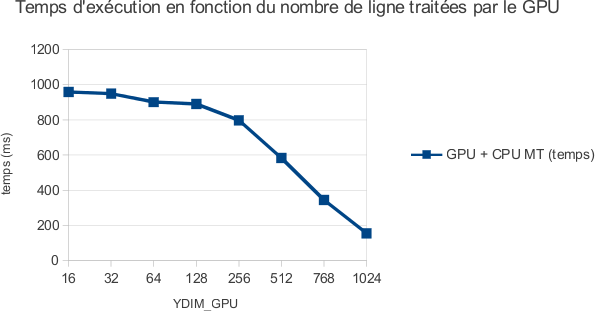
\includegraphics[scale=1.0]{temps}
		\end{figure}
	
		\begin{figure}[H]
			\centering
			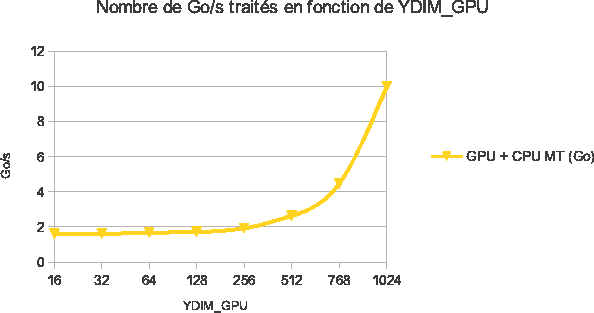
\includegraphics[scale=1.0]{go}
		\end{figure}

On peut voir ici que la version exécutée entièrement au GPU est la plus efficiente. 		
	\subsubsection{Machine du CREMI}
	
	Voici ensuite les mêmes graphes, mais tirés de l'exécution sur les machines du CREMI.
	
	\begin{figure}[H]
			\centering
			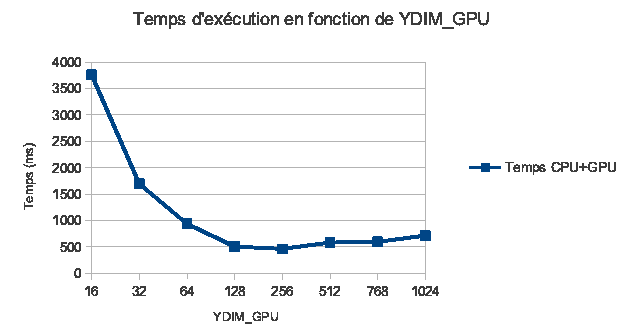
\includegraphics[scale=1.0]{tps_cremi.png}
		\end{figure}
	
		\begin{figure}[H]
			\centering
			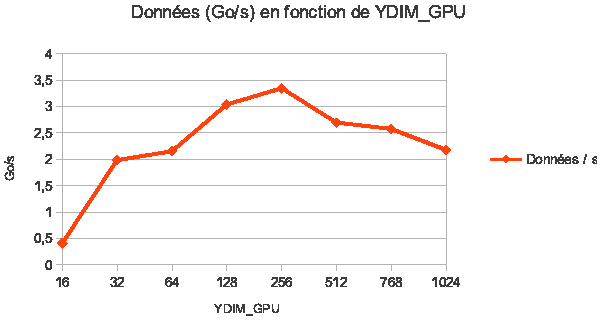
\includegraphics[scale=1.0]{go_cremi.png}
		\end{figure}

On voit par contre ici que le point optimal est atteint lorsque le GPU a 256 lignes à traiter.

La différence entre les deux tests peut s'expliquer par la configuration des machines. En effet, notre machine dispose de 384 coeurs CUDA, contre 96 
machines du CREMI. A l'opposé, ces dernières possède 8 coeurs CPU cadencé à 2.4GHz, hyper-threadés, alors que nous n'avions que 4 coeurs, certes cadencé à 3.3Ghz, mais non hyper-threadés. Ainsi, sur les machines du CREMI, le CPU pallie le manque de performance du GPU.